\begin{figure}[htbp]
\section*{ SUOX}
\centering
\begin{subfigure}[b]{0.5\textwidth}
\centering
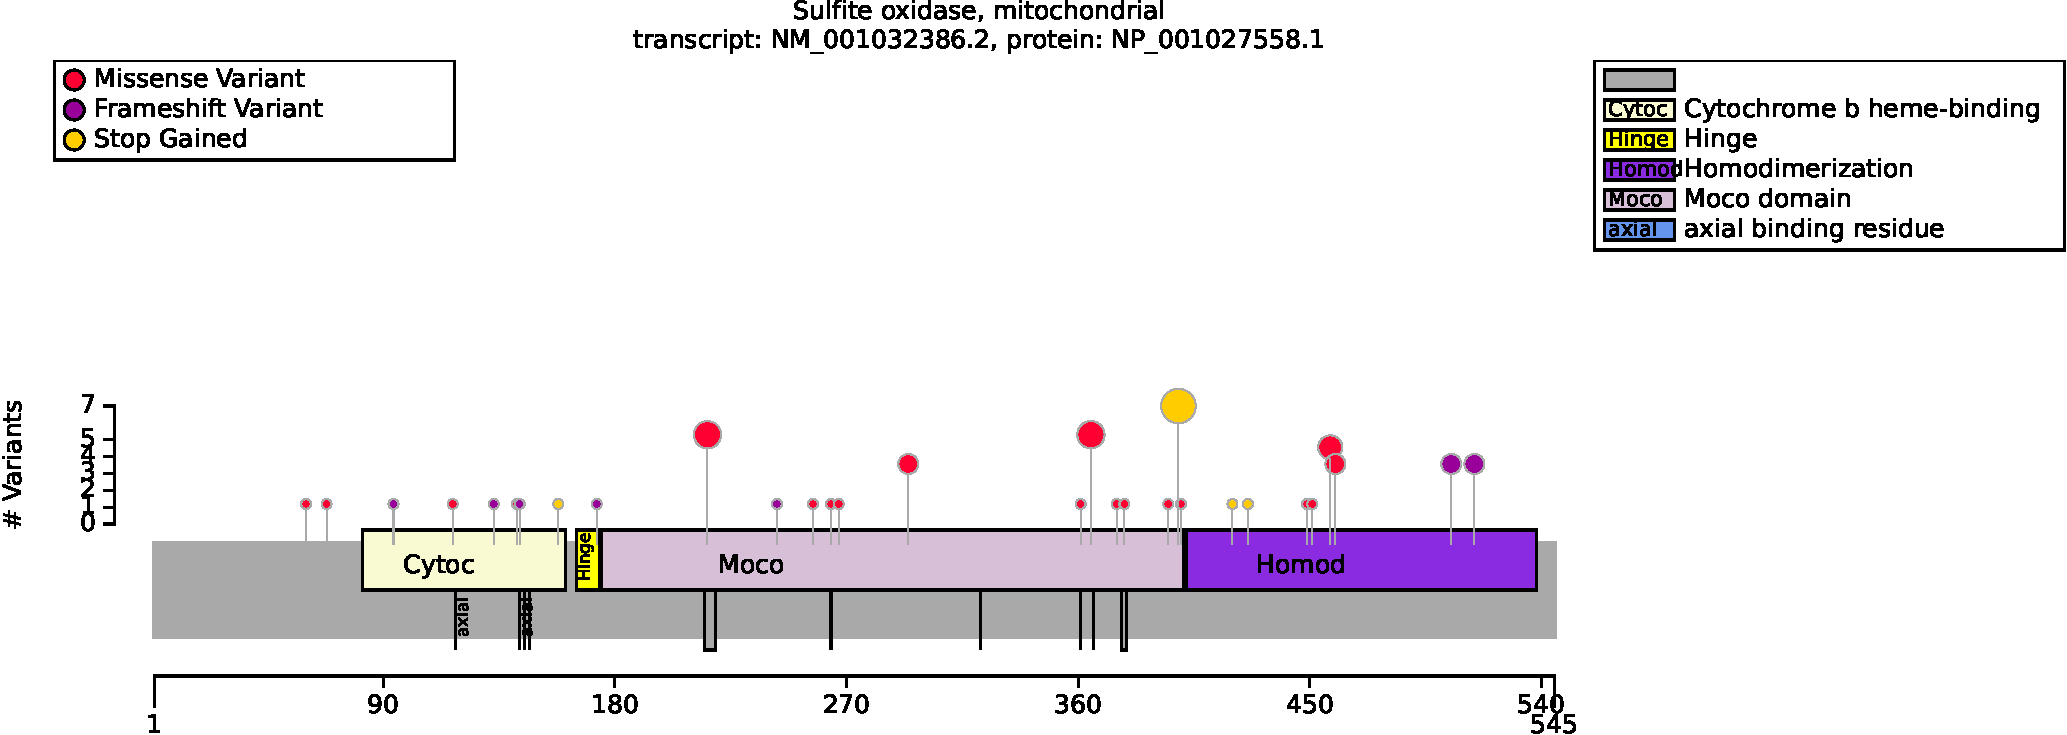
\includegraphics[width=\textwidth]{ img/SUOX_protein_diagram.pdf} 
\captionsetup{justification=raggedright,singlelinecheck=false}
\caption{Distribution of variants in SUOX}
\end{subfigure}
\begin{subfigure}[b]{0.45\textwidth}
\centering
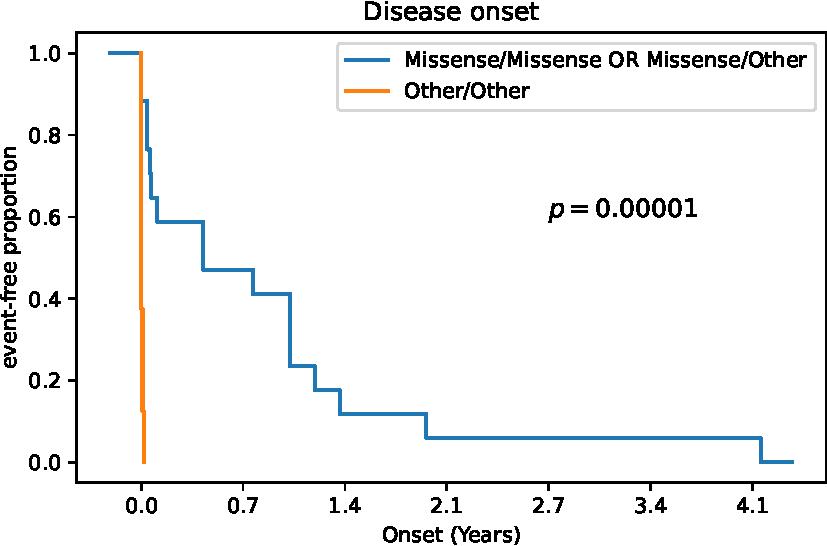
\includegraphics[width=\textwidth]{ img/SUOX_stats.pdf} 
\captionsetup{justification=raggedright,singlelinecheck=false}
\caption{Survival analysis: SUOX missense variants and disease onset}
\end{subfigure}

\vspace{2em}

\begin{subfigure}[b]{0.95\textwidth}
\centering
\resizebox{\textwidth}{!}{
\begin{tabular}{llllrr}
\toprule
HPO term & homodimerization/homodimerization OR homodimerization/Other & Other/Other & p-value & adj. p-value\\
\midrule
Microcephaly [HP:0000252] & 0/9 (0\%) & 10/12 (83\%) & $2.21\times 10^{-4}$ & 0.003\\
\bottomrule
\end{tabular}
}
\captionsetup{justification=raggedright,singlelinecheck=false}
\caption{Fisher Exact Test performed to compare HPO annotation frequency with respect to homodimerization/homodimerization OR homodimerization/Other and Other/Other. Total of
        15 tests were performed. }
\end{subfigure}
\vspace{0.2em}
\begin{subfigure}[b]{0.95\textwidth}
\centering
\resizebox{\textwidth}{!}{
\begin{tabular}{llllrr}
\toprule
Genotype (A) & Genotype (B) & total tests performed & significant results\\
\midrule
Missense/Missense OR Missense/Other & Other/Other & 14 & 0\\
Moco domain/Moco domain OR Moco domain/Other & Other/Other & 14 & 0\\
\bottomrule
\end{tabular}
}
\captionsetup{justification=raggedright,singlelinecheck=false}
\caption{Fisher Exact Test performed to compare HPO annotation frequency with respect to genotypes. }
\end{subfigure}

\vspace{0.2em}

\begin{subfigure}[b]{0.95\textwidth}
\captionsetup{justification=raggedright,singlelinecheck=false}
\resizebox{\textwidth}{!}{
\begin{tabular}{llllrr}
\toprule
Description & Variable & Genotype (A) & Genotype (B) & p-value & xrefs\\
\midrule
Onset of Sulfite oxidase deficiency (OMIM:272300) & Onset of OMIM:272300 & Missense/Missense OR Missense/Other & Other/Other & $9.18\times 10^{-6}$ & -\\
\bottomrule
\end{tabular}
}
\caption{ Onset of OMIM:272300 to compare Missense/Missense OR Missense/Other and Other/Other with respect to Onset of OMIM:272300. }
\end{subfigure}

\vspace{0.2em}

\begin{subfigure}[b]{0.95\textwidth}
\captionsetup{justification=raggedright,singlelinecheck=false}
\resizebox{\textwidth}{!}{
\begin{tabular}{llllrr}
\toprule
Description & Variable & Genotype (A) & Genotype (B) & p-value & xrefs\\
\midrule
Onset of Sulfite oxidase deficiency (OMIM:272300) & Onset of OMIM:272300 & homodimerization/homodimerization OR homodimerization/Other & Other/Other & 0.853 &\cite{PMID_36303223}\\
\bottomrule
\end{tabular}
}
\caption{ Onset of OMIM:272300 to compare homodimerization/homodimerization OR homodimerization/Other and Other/Other with respect to Onset of OMIM:272300. }
\end{subfigure}

\vspace{0.2em}

\caption{ The cohort comprised 35 individuals (11 females, 14 males, 10 with unknown sex). 8 of these individuals were reported to be deceased. 
A total of 20 HPO terms were used to annotate the cohort. Disease diagnosis: Sulfite oxidase deficiency (OMIM:272300). 
A published Genotype-phenotype analysis demonstrated patients with biallelic missense mutations 
had milder symptoms (P = 0.023), later age of onset (P $<$ 0.001), and a higher incidence of regression (P = 0.017)
than other genotypes \cite{PMID_36303223}. A total of 48 unique variant alleles were found in \textit{SUOX} (transcript: \texttt{NM\_001032386.2}, protein id: \texttt{NP\_001027558.1}).}
\end{figure}
